\documentclass[12pt]{article}
\usepackage{tikz}
\usepackage[a0paper,top=1.2cm,bottom=1cm,left=0.8cm,right=0.8cm]{geometry}
\usepackage[fontsize=24pt]{fontsize}
\usepackage{etoolbox}
\usepackage[utf8]{inputenc}
\usepackage[T1]{fontenc}
\usepackage{lmodern}
\usepackage[scaled=1.08]{helvet}
\renewcommand{\familydefault}{\sfdefault}
\usepackage{parskip}
\usepackage{microtype}
\usepackage{amsmath,amsthm,amssymb,amsfonts, enumitem, fancyhdr, color, graphicx, environ}
\usepackage{wrapfig}
\usepackage{tcolorbox}
\tcbuselibrary{poster}
\usepackage{colortbl}
\usetikzlibrary{positioning}

\pagenumbering{gobble}
\newtheorem{defin}{Definition}
\newtheorem{theom}{Theorem}
\newtheorem{propos}{Proposition}
\newtheorem{lemm}{Lemma}
\definecolor{PosterBg}{RGB}{235,241,255}
\definecolor{PosterBand}{RGB}{20,82,143}
\definecolor{PosterBandSoft}{RGB}{78,134,194}
\definecolor{PosterAccent}{RGB}{246,159,67}
\definecolor{PosterText}{RGB}{22,36,58}
\definecolor{PosterBorder}{RGB}{117,154,199}

\begin{document}
\thispagestyle{empty}

\begin{tikzpicture}[remember picture,overlay]
    \fill[PosterBg] (current page.south west) rectangle (current page.north east);
    \shade[top color=PosterBandSoft!92,bottom color=PosterBand] ([yshift=-1.8cm]current page.north west) rectangle ([yshift=-9.2cm]current page.north east);
    \fill[white,opacity=0.16] ([yshift=-1.8cm,xshift=2cm]current page.north west) rectangle ([yshift=-5.1cm,xshift=26cm]current page.north west);
    \fill[white] ([yshift=-9.2cm]current page.north west) rectangle ([yshift=-9.55cm]current page.north east);
    \fill[PosterAccent] ([yshift=-9.55cm]current page.north west) rectangle ([yshift=-10cm]current page.north east);
\end{tikzpicture}

\vspace{-1.8cm}
\begin{center}
\begin{tabular}{p{3.5cm}p{\paperwidth-7cm}p{3.5cm}}
\vspace{-3cm} & & \vspace{-3cm}\hspace{-2cm}
\includegraphics[width=3cm,height=2.2cm]{source/logo-name.pdf} \\
\end{tabular}
\end{center}

\vspace{-5cm}
\begin{center}
    {\color{white}\changefontsize{40pt}{\textbf{On the Limitations of the Modulo Trick Method in Solving Exponential Diophantine Equations of the Form $\boldsymbol{1+p^a=q^b+r^c}$}}} \\
    \vspace{0.25cm}
    {\color{white!92}\noindent\rule{49cm}{0.3pt}}
    
    {\color{white}\changefontsize{21pt}{Burapat Suwanprasert$^{1}$, Kawin Chumtong$^{1}$, Kijti Rodtes$^{2}$ \\
    $^{1}$Naresuan University Secondary Demonstration School, Thailand \\
    $^{2}$Department of Mathematics, Faculty of Science, Naresuan University, Thailand}}
\end{center}

\vspace{1.25cm}

\tcbset{
fontupper=\fontsize{18pt}{22pt}\selectfont,
colback=white,
colframe=PosterBorder,
boxrule=1.2pt,
arc=4mm,
left=6mm,
right=6mm,
top=4mm,
bottom=4mm,
title filled=true,
colbacktitle=PosterBand,
coltitle=white,
fonttitle=\bfseries\fontsize{20pt}{24pt}\selectfont,
drop fuzzy shadow=black!18!white,
before skip=2mm,
after skip=2mm,
}

\begin{tcbposter}[
poster = {showframe=false,columns=3,rows=6,spacing=7mm,height=84cm},
]

\posterbox[adjusted title=Abstract]{name=abstract,span=3,below=top}{
\textbf{Background:} The resolution of exponential Diophantine equations has historically relied on elementary congruence methods versus sophisticated analytical tools like Baker's theory. Among the most accessible elementary techniques is the \textbf{modulo trick}, which uses carefully selected moduli to establish congruences that bound or eliminate potential solution sets.

\textbf{Problem:} Brenner and Foster (1982) noted certain equation forms "seem not amenable" to this method, but no rigorous framework existed to prove such impossibility.

\textbf{Objective:} This research formalizes "solvable with modulo trick" and proves limitations for specific equation structures.

\textbf{Main Contributions:} (1) First rigorous definitions of solvability/non-solvability via modulo trick. (2) Proved $1+(pq)^a = p^b + q^c$ is non-solvable for coprime $p,q$. (3) Proved $a^x-a^y = b^z-b^w$ is non-solvable for any $a,b$. (4) Validated Brenner and Foster's heuristic observations.

\textbf{Significance:} Provides a diagnostic tool for researchers to determine when elementary modular methods are fundamentally inadequate, necessitating advanced techniques like Baker's theory of linear forms in logarithms.
}

\posterbox[adjusted title=Background and Significance]{name=bg,column=1,row=1}{
\textbf{Historical Context}

The study of exponential Diophantine equations---where unknowns appear in exponents---has been a cornerstone of number theory. A celebrated example is Catalan's Conjecture ($x^a - y^b = 1$), proposed in 1844 and proved by Mihăilescu in 2002 using cyclotomic fields and linear forms in logarithms.

\textbf{The Modulo Trick Method}

In practice, many researchers first attempt to solve these equations using the \textbf{modulo trick}:
\begin{enumerate}
    \item Choose a modulus $m$
    \item Establish congruence: $1+p^a \equiv q^b+r^c \pmod{m}$
    \item This restricts possible values of exponents
    \item Repeat with additional moduli until solutions are bounded
\end{enumerate}

Brenner and Foster (1982) successfully applied this method to numerous equations of the form $1+p^a = q^b + r^c$ with specific values of $p,q,r$.

\textbf{The Gap}

However, they remarked that certain classes:
\[(pq)^x - p^y - q^z + 1 = 0 \quad \text{and} \quad p^x - p^y + q^z - q^w = 0\]
"seem not amenable" to their congruence-based methods, but provided no rigorous proof.
}

\posterbox[adjusted title=Rationale for the Study]{name=rationale,column=2,row=1}{
\textbf{Why This Research Matters}

The literature lacked:
\begin{itemize}
    \itemsep0.1cm
    \item A \textbf{formal definition} of what it means for an equation to be "solvable with modulo trick"
    \item A \textbf{rigorous proof} of why certain equations resist modular treatment
    \item A \textbf{mathematical framework} to characterize when the method succeeds or fails
\end{itemize}

\textbf{Research Questions}

\begin{enumerate}
    \item What does it mean for an equation to be "solvable by modulo trick"?
    \item Why are some equations "non-solvable" by this method?
    \item Can we prove the non-solvability of cases Brenner and Foster observed?
\end{enumerate}

\textbf{Our Approach}

We bridge the gap between heuristic observations and formal impossibility proofs by:
\begin{itemize}
    \itemsep0.1cm
    \item Introducing precise mathematical definitions
    \item Developing a formal framework for the modulo trick
    \item Proving non-solvability for specific equation families
    \item Validating prior research observations
\end{itemize}
}

\posterbox[adjusted title=Research Objectives]{name=objectives,column=3,row=1}{
\textbf{Main Goal:} Turn the modulo trick from a useful idea into a precise method we can test, prove, and apply.

\vspace{0.2cm}
\begin{tcolorbox}[colback=blue!15, colframe=blue!60!black]
\textbf{Objective 1: Define} \\
Formalize "solvable with modulo trick" and "non-solvable with modulo trick" based on whether the method yields a bounded solution set.
\end{tcolorbox}

\vspace{0.15cm}
\begin{tcolorbox}[colback=green!15, colframe=green!60!black]
\textbf{Objective 2: Build} \\
Develop a mathematical framework that models the modulo trick method using sets and congruences.
\end{tcolorbox}

\vspace{0.15cm}
\begin{tcolorbox}[colback=orange!15, colframe=orange!60!black]
\textbf{Objective 3: Prove} \\
Establish rigorous proofs showing when the modulo trick method fails for specific equation families.
\end{tcolorbox}

\vspace{0.15cm}
\begin{tcolorbox}[colback=purple!15, colframe=purple!60!black]
\textbf{Objective 4: Validate} \\
Confirm Brenner and Foster's heuristic observations with mathematical proofs.
\end{tcolorbox}
}

\posterbox[adjusted title=Methodology]{name=method,column=1,span=2,below=bg}{
\textbf{Mathematical Framework Development}

\textbf{Step 1: Computability Proposition} \\
We first establish when an equation is "computable" (all solutions accessible in finite time):

\vspace{0.1cm}
\begin{tcolorbox}[colback=red!10, colframe=red!60!black]
\begin{propos}
Equation $1+p^a = q^b + r^c$ is computable if at least one condition holds:
\begin{enumerate}
    \item $\exists M$ such that $a \leq M$ for any solution $(a,b,c)$
    \item $\exists M_b, M_c$ such that $b \leq M_b$ and $c \leq M_c$ for any solution
\end{enumerate}
\end{propos}
\end{tcolorbox}

\textbf{Step 2: Define Solution Sets} \\
Let $m_1,m_2,...,m_k$ be moduli used. Define:
\[S_0^{p,q,r} = \mathbb{Z}_{\geq0}^3\]
\[S_i^{p,q,r} = \{(a,b,c)\in S_{i-1}^{p,q,r} \mid 1+p^a \equiv q^b+r^c \pmod{m_i}\}\]

\textbf{Step 3: Key Lemma (LCM Property)} \\
\vspace{0.1cm}
\begin{tcolorbox}[colback=blue!10, colframe=blue!60!black]
\begin{lemm}
For any moduli $m_1,...,m_k$:
\[S_k^{p,q,r} = \bigcap_{i=1}^k A_{m_i} = A_{\text{lcm}(m_1,...,m_k)}\]
\end{lemm}
\textbf{Significance:} Any sequence of moduli reduces to a single modulus (LCM).
\end{tcolorbox}

\textbf{Step 4: Formal Definitions} \\
Define "solvable" when finite moduli yield bounded solutions; "non-solvable" when unbounded solutions persist for any finite moduli choice.
}

\posterbox[adjusted title=Results - Theorem 1]{name=thm1,column=3,below=objectives}{
\begin{tcolorbox}[colback=purple!20, colframe=purple!80!black, center, title=\bfseries\selectfont Theorem 1 (Main Result)]
For fixed coprime $p,q \in \mathbb{N}\setminus\{1\}$:
\[1+(pq)^a = p^b + q^c\]
is \textbf{non-solvable with modulo trick}.
\end{tcolorbox}

\vspace{0.15cm}
\textbf{Proof Strategy:}

\begin{enumerate}\setlength{\itemsep}{0.05cm}
    \item Partition prime factors of any modulus $m$ into sets for $p$, $q$, and neither
    \item Factor $m = \chi \cdot \Gamma \cdot \mathrm{Z}$ where:
    \begin{itemize}
        \item $\chi$ contains primes dividing $p$
        \item $\Gamma$ contains primes dividing $q$
        \item $\mathrm{Z}$ contains primes dividing neither
    \end{itemize}
    \item Apply Euler's theorem with parameters $\theta_a, \theta_b, \theta_c$
    \item Construct solutions with arbitrarily large exponents
\end{enumerate}

\textbf{Corollary:} For distinct primes $p,q$, the equation is non-solvable with modulo trick.

\vspace{0.1cm}
\begin{tcolorbox}[colback=yellow!15, colframe=yellow!60!black]
\textbf{Significance:} This validates Brenner \& Foster's comment (8.037) that $1+(pq)^a = p^b+q^c$ "seems not amenable" to their method.
\end{tcolorbox}
}

\posterbox[adjusted title=Results - Theorem 2]{name=thm2,column=1,below=method}{
\begin{tcolorbox}[colback=teal!20, colframe=teal!80!black, center, title=\bfseries\selectfont Theorem 2 (Generalization)]
For $a,b \in \mathbb{Z}^+$:
\[a^x - a^y = b^z - b^w\]
is \textbf{non-solvable with modulo trick}.
\end{tcolorbox}

\vspace{0.15cm}
\textbf{Key Lemma (Period of Exponent Residues):}
\vspace{0.1cm}
\begin{tcolorbox}[colback=blue!10, colframe=blue!60!black]
\begin{lemm}
The sequence $(a^x \bmod n)_{x=1}^\infty$ is eventually periodic. That is, $\exists k,\epsilon \in \mathbb{Z}_{\geq 0}$ such that:
\[a^x \equiv a^{x+\epsilon} \pmod n \quad \forall x \geq k\]
\end{lemm}
\textbf{Proof:} Uses pigeonhole principle on the finite set $\{0,1,...,n-1\}$.
\end{tcolorbox}

\textbf{Proof of Theorem 2:}
\begin{enumerate}\setlength{\itemsep}{0.05cm}
    \item For any modulus $d$, Lemma 8 gives periods $\epsilon_a, \epsilon_b$
    \item For any $x \geq k_a, y \geq k_b$:
    \[(x,\; x+N\epsilon_a,\; y,\; y+M\epsilon_b) \in A'_d\]
    \item These can be made arbitrarily large
\end{enumerate}

\textbf{Corollary:} For distinct primes $p,q$: $p^x - p^y = q^z - q^w$ is non-solvable (validates Brenner \& Foster 8.033).
}

\posterbox[adjusted title=Methodology Flowchart]{name=flow,column=2,below=method}{
\textbf{Research Methodology Flowchart:}

\vspace{0.2cm}
\scalebox{0.5}{
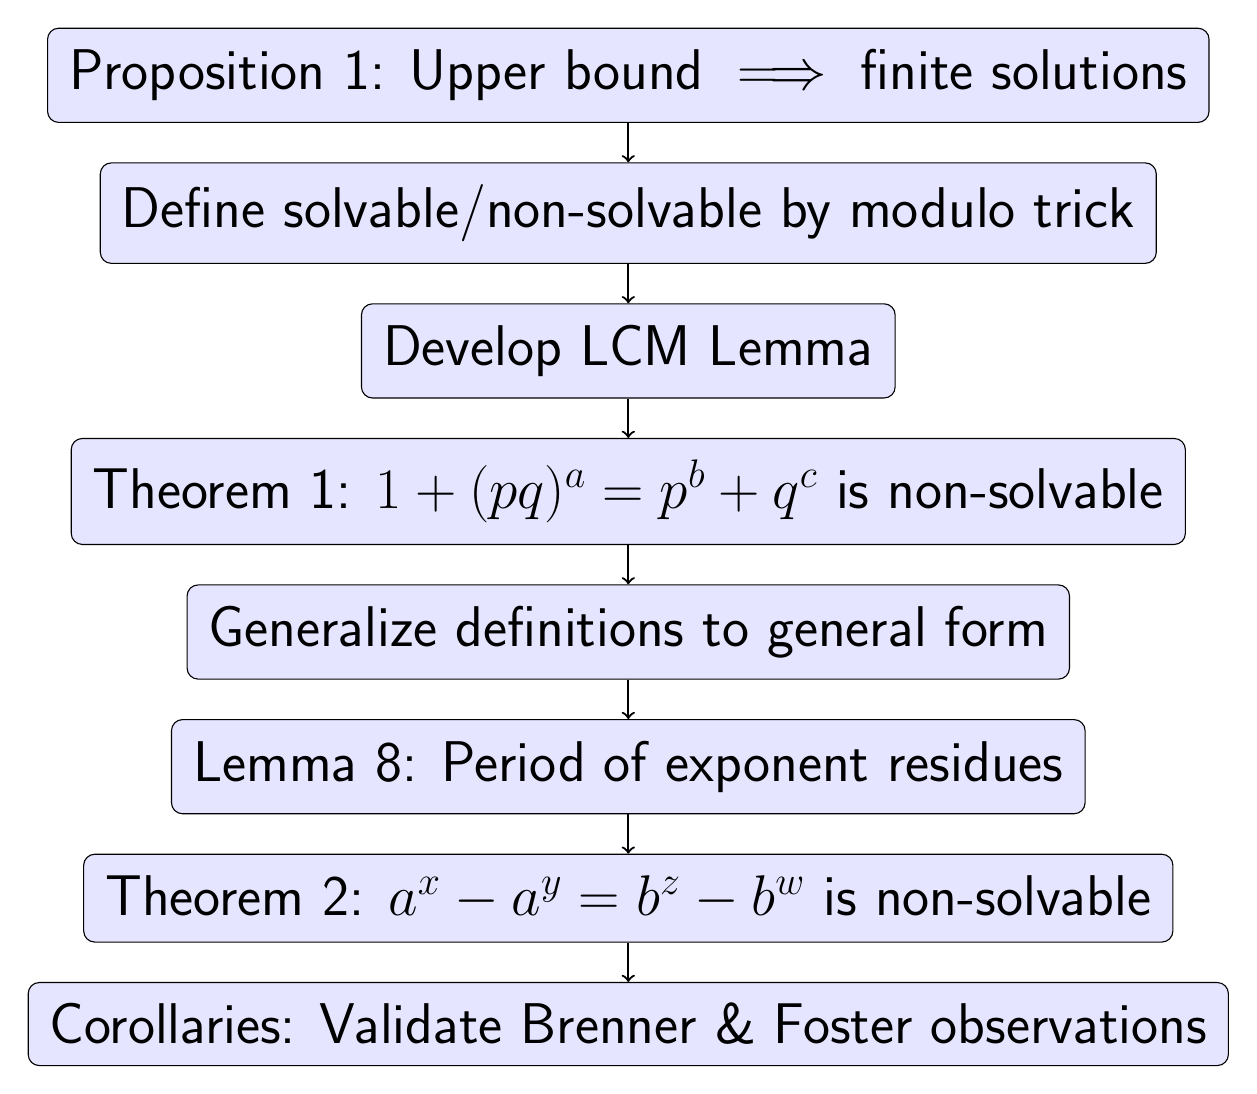
\begin{tikzpicture}[
    node distance=0.5cm,
    box/.style={rectangle, draw, rounded corners, align=center, minimum width=4.5cm, minimum height=0.7cm, fill=blue!10, font=\small},
    arrow/.style={->, thick}
]
\node[box] (1) {Proposition 1: Upper bound $\implies$ finite solutions};
\node[box, below=of 1] (2) {Define solvable/non-solvable by modulo trick};
\node[box, below=of 2] (3) {Develop LCM Lemma};
\node[box, below=of 3] (4) {Theorem 1: $1+(pq)^a = p^b+q^c$ is non-solvable};
\node[box, below=of 4] (5) {Generalize definitions to general form};
\node[box, below=of 5] (6) {Lemma 8: Period of exponent residues};
\node[box, below=of 6] (7) {Theorem 2: $a^x-a^y = b^z-b^w$ is non-solvable};
\node[box, below=of 7] (8) {Corollaries: Validate Brenner \& Foster observations};
\draw[arrow] (1) -- (2);
\draw[arrow] (2) -- (3);
\draw[arrow] (3) -- (4);
\draw[arrow] (4) -- (5);
\draw[arrow] (5) -- (6);
\draw[arrow] (6) -- (7);
\draw[arrow] (7) -- (8);
\end{tikzpicture}}

\vspace{0.3cm}
\textbf{Key Insight:} The modulo trick succeeds exactly when the congruence conditions eventually force all solutions into a bounded set.
}

\posterbox[adjusted title=Conclusion and Summary of Findings]{name=conclusion,column=3,below=thm1}{
\textbf{Summary of Contributions:}

\begin{enumerate}\setlength{\itemsep}{0.1cm}
    \item \textbf{First rigorous definitions} of "solvable/non-solvable with modulo trick"
    \item \textbf{Mathematical framework} using solution sets $S_k^{p,q,r}$ and LCM lemma
    \item \textbf{Theorem 1:} Proved $1+(pq)^a = p^b+q^c$ is non-solvable for coprime $p,q$
    \item \textbf{Theorem 2:} Proved $a^x-a^y = b^z-b^w$ is non-solvable for any $a,b$
    \item \textbf{Corollaries} validating Brenner and Foster's heuristic observations
\end{enumerate}

\vspace{0.2cm}
\begin{tcolorbox}[colback=green!15, colframe=green!60!black]
\textbf{Practical Recommendations:}

For equations of the forms:
\begin{itemize}
    \itemsep0.05cm
    \item $1+(pq)^a = p^b + q^c$
    \item $a^x - a^y = b^z - b^w$
\end{itemize}

\textbf{Do NOT} use the modulo trick. Instead, proceed directly to:
\begin{itemize}
    \itemsep0.05cm
    \item Baker's theory of linear forms in logarithms
    \item Upper bounds from Tijdeman and Wang (1988)
    \item Advanced computational methods
\end{itemize}
\end{tcolorbox}

\vspace{0.2cm}
\textbf{Future Research Directions:}
\begin{itemize}
    \itemsep0.05cm
    \item Find non-trivial equations that ARE solvable with modulo trick
    \item Develop complete characterization of solvability conditions
    \item Apply framework to other forms of exponential Diophantine equations
    \item Investigate connections to Baker's theory
\end{itemize}
}

\posterbox[adjusted title=Acknowledgements]{name=ack,column=1,span=2,above=bottom}{
\textbf{Acknowledgements:}

\begin{tabular}{p{6.5cm}p{6.5cm}p{6cm}}
\textbf{Academic Support:} & \textbf{Institutional Support:} & \textbf{Personal Support:} \\
\begin{itemize}
    \setlength{\itemsep}{0.05cm}
    \item Assoc. Prof. Dr. Kijti Rodtes (Research Advisor)
    \item Department of Mathematics, Faculty of Science
    \item Naresuan University
\end{itemize} &
\begin{itemize}
    \setlength{\itemsep}{0.05cm}
    \item Science Classrooms in University-Affiliated School Project (SCiUS)
    \item Naresuan University Secondary Demonstration School
    \item Research facilities and resources
\end{itemize} &
\begin{itemize}
    \setlength{\itemsep}{0.05cm}
    \item Our families for unwavering support
    \item Friends at SCiUS for the wonderful environment
    \item All who contributed to this research
\end{itemize}
\end{tabular}

\vspace{0.2cm}
\textbf{Contact Information:} \\
Burapat Suwanprasert (Student ID: 67983443) \hspace{0.5cm} Kawin Chumtong (Student ID: 67983115) \\
SCiUS, Naresuan University Secondary Demonstration School, Phitsanulok, Thailand
}

\posterbox[adjusted title=References]{name=refs,column=3,above=bottom}{
\textbf{References:}

\begin{enumerate}\setlength{\itemsep}{0.05cm}\small
    \item J. L. Brenner and L. L. Foster, "Exponential Diophantine Equations," \textit{Pacific J. Math.}, vol. 101, no. 2, pp. 263-301, 1982.
    \item L. Wang and R. Tijdeman, "Exponential Diophantine Equations with Four Terms," \textit{Indag. Math.}, vol. 51, pp. 89-96, 1988.
    \item M. Deze and R. Tijdeman, "Exponential Diophantine Equations with Four Terms," \textit{Indagationes Mathematicae}, vol. 3, no. 1, pp. 47-57, 1992.
    \item T. N. Shorey and R. Tijdeman, \textit{Exponential Diophantine Equations}, Cambridge University Press, 1986.
    \item P. Mihăilescu, "Primary Cyclotomic Units and a Proof of Catalan's Conjecture," \textit{J. Reine Angew. Math.}, vol. 572, pp. 167-195, 2004.
\end{enumerate}
}

\posterbox[adjusted title=Keywords]{name=keywords,column=1,span=3,below=bottom}{
\begingroup
\vspace{-0.3cm}
\textbf{Keywords:} Exponential Diophantine Equations $\cdot$ Modulo Trick $\cdot$ Modular Arithmetic $\cdot$ Non-solvability Proofs $\cdot$ Baker's Theory $\cdot$ Brenner and Foster
\endgroup
}

\end{tcbposter}

\end{document}
